\section{Implementation}\label{implementation}

The following sections describe the implementation of the workflow system.
First of all the integration of WS-PGRADE/gUSE with the existing cloud architecture is described, followed by the configuration and trouble shooting of the system.
The last section explains different approaches to create workflows built on top of a sample application.

\subsection{Architecture}\label{architecture}

The existing QM-ROCT server infrastructure consists of various system components (see figure~\ref{fig:architecture}), which are loosely coupled as web services.
A server machine running an instance of XNAT can be accessed via the internet, so that researchers are able to upload and manage data using the graphical web interface.
Other components of the architecture are encapsulated in a private network.
Especially the OpenStack cloud is not reachable from the internet. The only accesspoint for XNAT, to send data processing jobs to the cloud, is a gateway server running a REST web-service.
The gateway server is responsible for communicating with the cloud control server to start a Virtual Machine, submit the incoming job and stop the VM again, when the processing is done.
When submitting a job from XNAT, using the XNAT pipeline system (see section~\ref{xnat}), no data files are transferred to the gateway server.
Only parameters are transferred, which are used to download the files via the XNAT Rest API.
the download happens inside the VM, which connects to XNAT for downloading data and for uploading the results.
This ensures, that no unnecessary file transfers are performed. 

When introducing gUSE to this infrastructure it is important to deploy it inside the private network, because the DCI bridge communicates with the VM instances directly in order to orchestrate them.
As can be seen in figure~\ref{fig:architecture} the web interface is accessible via the internet, so that application developers can create new workflows.
The data processing requests are still being sent to the gateway server, which forwards this request to the gUSE Rest API (see section~\ref{guse}).
The gateway server is not in charge of communicating with OpenStack anymore.
The workflow system manages data transfers on its own, so that the data files should be downloaded before the workflow starts, which results in more data transfers.
This approach and two alternative workflow implementations are further described in section~\ref{workflowimplementation}.

\begin{figure*}%[!b]
                \centering
                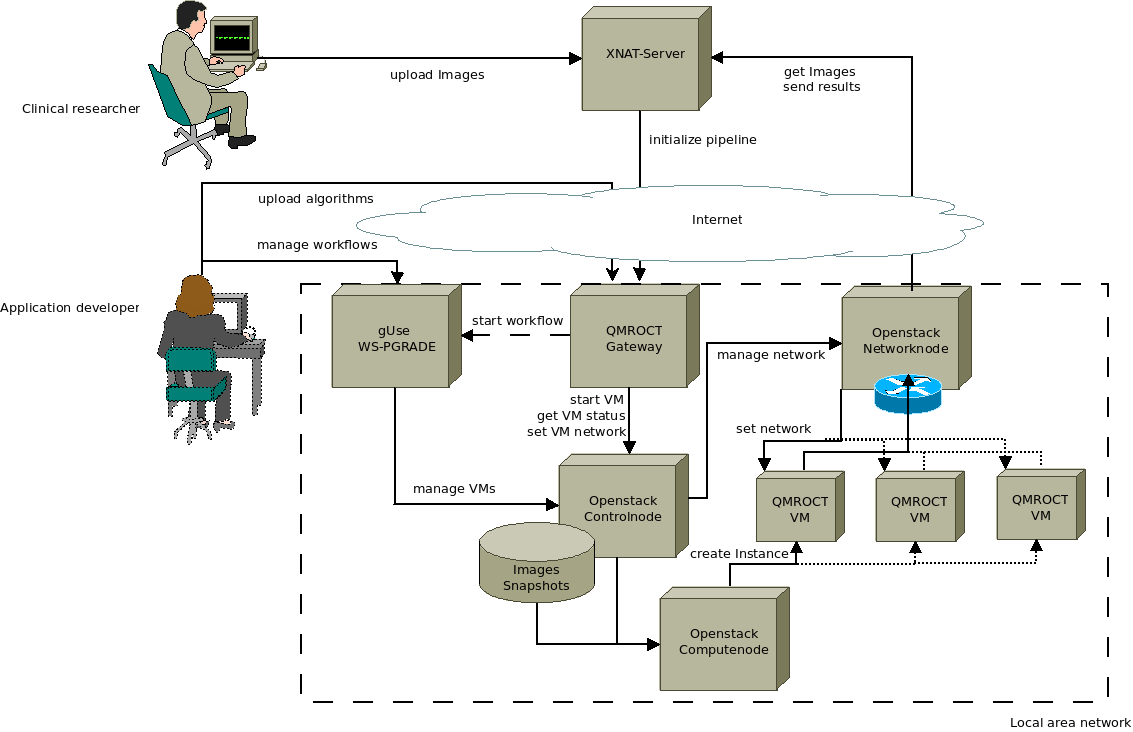
\includegraphics[width=2.0\columnwidth]{images/somno-architecture.png}
                \caption{Architecture of QM-ROCT \cite{wu14} including WS-PGRADE/gUSE}
                \label{fig:architecture}
\end{figure*}

\subsection{Configuration}\label{configuration}

The cloud plugin of the DCI bridge ships with gUSE and is activated by default.

A new configuration, as can be seen in figure~\ref{fig:cloudconfig}, is created in the web interface under \textit{Information, Resources, Cloud}.
In this case the name of the configuration is set as \textit{local cloud} and the status is \textit{enabled}. The field \textit{service and parameters} specifies three important settings.
The first part is the URL referencing the EC2 interface of OpenStack and can be found in the OpenStack web interface under \textit{Access \& Security, API Access}.
The second parameter is the EC2 ID of the image or snapshot the Virtual Machine is based on.
This EC2 ID is not the same as the ID listed in the OpenStack web interface, which is only suitable for the Nova API.
The EC2 ID can be determined by using the euca2ools command \textit{euca-describe-instances}.
The third parameter is the maximum number of VM instances managed at once.
This number should not be higher than the number of instances that can actually be handled by the given cloud resources.
gUSE will not determine the load of the cloud.

After creating the new cloud configuration the security credentials must be given under \textit{security, cloud, local cloud}.
The EC2 credentials for OpenStack can be downloaded from the OpenStack EC2 web interface under \textit{Access \& Security, API Access, Download EC2 Credentials}.
The downloaded archive contains a text file named \textit{ec2rc.sh}, which contains the necessary values.
The value of the variable \textit{EC2\_ACCESS\_KEY} maps to the user field and \textit{EC2\_SECRET\_KEY} maps to the password field of gUSE.

\begin{figure*}%[!b]
                \centering
                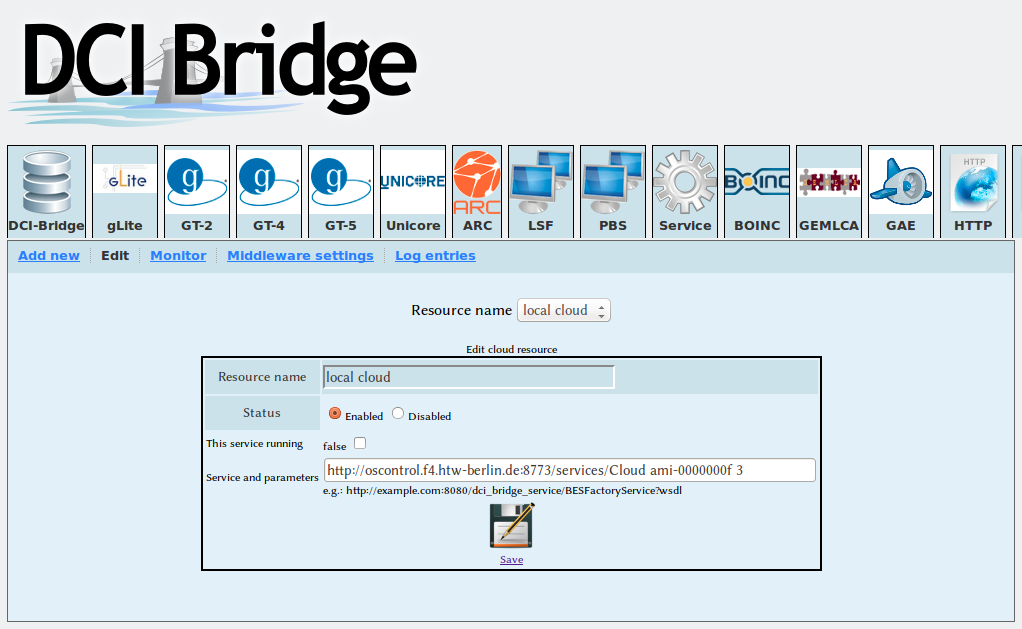
\includegraphics[width=2.0\columnwidth]{images/dci-cloud-settings.png}
                \caption{DCI cloud configuration}
                \label{fig:cloudconfig}
\end{figure*}

With the given information gUSE is able to run euca2ools commands in order to create and terminate VM instances and to determine the IP address of a running VM.
A problem that occurred with euca2ools in the private network is the wrong assignment of public IP addresses.
The public IP address, that got assigned was not reachable inside the network and therefore not usable.
The solution to this problem are customized start and terminate scripts \cite{customscripts} which use Nova tools(see section~\ref{euca}) instead of the EC2 API.
These customized scripts replace the programs \textit{euca-run-instances} and \textit{euca-terminate-instances} in the directory \textit{/usr/bin} of the gUSE server.
The start script manually assigns a floating IP to the VM instance, instead of using the automatic public IP assignment of OpenStack.

\subsection{Workflows}\label{workflowimplementation}

The sample application described in section~\ref{applications} is used to model workflows in the WS-PGRADE web interface.
The basic workflow \cite{somnocqrs} describes the two algorithms FD1\_AF2\_DF2 and CQRS as two seperated jobs (see figure~\ref{fig:CQRSworkflow}).
The FD1\_AF2\_DF2 job has two input ports, describing the ecg.hea and ecg.dat files.
These files are necessary inputs for the algorithm.
The job has five output ports, which are connected to the input ports of the CQRS job.
These five ports handle the data transfer between both jobs for the two original files ecg.hea and ecg.dat, as well as for three newly created files ecg\_fd1.dat, ecg\_af2.dat and ecg\_df2.dat.
The CQRS job has one output port, which describes the final output file cqrs.dat produced by the algorithm.

The input files must be given to the workflow management system before the processing starts.
This means that the data files must be transferred to the gUSE server, for example by automatically downloading them from XNAT.
The workflow manager transfers the data to a Virtual Machine and processes the algorithm.
All five output files are transferred back to the gUSE server and then copied to a another VM to process the second job.
Also the final result file needs to be transferred back to the gUSE server.
In order to reduce the number of file transfers, the workflow can be modeled in different ways.

Instead of handling the input and output files with the workflow manager, the results can be downloaded from XNAT directly to the Virtual Machine where the processing takes place.
For this purpose a download script has been written, which is included with the algorithm scripts and binaries.
The CQRS download workflow~\cite{somnocqrsdl}, as can be seen in figure~\ref{fig:CQRSDLworkflow}, has only one input port.
This input port takes a text file including download parameters, which are used to connect to the XNAT server for downloading the actual input files.
The output ports of the first job include the same five files as the basic workflow.
The sixth output port additionally transfers the parameter file to the second job.
When the second job is processed, the result file is not being handled by gUSE, but gets uploaded to XNAT.
This workflow reduces the number of file transfers, but the outputs of the first job are still transferred to the gUSE server and then to another VM for the second job.

When gUSE should not handle file transfers at all, both algorithms can be modeled as one job~\cite{somnocqrsone} (see figure~\ref{fig:CQRSONEworkflow}).
The third workflow includes both algorithms in one job and takes only one input, a parameter file.
The only file transfers are the download from XNAT and the upload of the result file.
Unfortunately the main benefit of the workflow system is lost, because the intermediate results are not stored by gUSE and both algorithms must be processed again, if something fails.
But for small algorithms with a short processing time, this kind of workflow modeling can still be a better option, because the file transfers take longer than the processing itself.

\begin{figure*}%[!b]
                \centering
                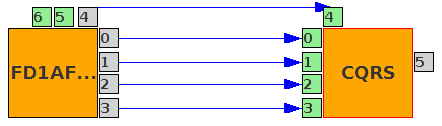
\includegraphics[width=1.0\columnwidth]{images/SOMNO_CQRS.png}
                \caption{SOMNO CQRS workflow}
                \label{fig:CQRSworkflow}
\end{figure*}

\begin{figure*}%[!b]
                \centering
                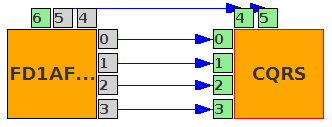
\includegraphics[width=0.8\columnwidth]{images/SOMNO_CQRS_DL_SAMPLE.png}
                \caption{SOMNO CQRS workflow with XNAT data download}
                \label{fig:CQRSDLworkflow}
\end{figure*}

\begin{figure*}%[!b]
                \centering
                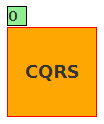
\includegraphics[width=0.3\columnwidth]{images/SOMNO_CQRS_ONE_SAMPLE.png}
                \caption{SOMNO CQRS workflow with XNAT data download and only one job}
                \label{fig:CQRSONEworkflow}
\end{figure*}